\section{Introdução e contexto histórico}

\frame{
	\frametitle{Como descobriu-se a eletricidade?}
	\begin{block}{Tales de Mileto}
		\begin{itemize}
			\item Século VI a.C., na Grécia Antiga.
			\item Descobre que ao se esfregar âmbar (resina vegetal fóssil petrificada) com pele de carneiro, observa-se que pedaços de palha e penas eram atraídos pelo âmbar.
		\end{itemize}
	\end{block}
	\centerline{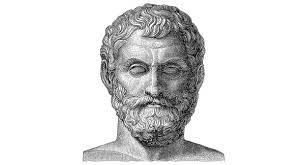
\includegraphics[width=0.7\linewidth]{Figuras/Ch01/mileto.jpg}}
}

\frame{
	\frametitle{Como descobriu-se a eletricidade?}
	\begin{block}{O experimento de Mileto}
		\begin{itemize}
			\item A palavra eléktron significa âmbar em grego.
		\end{itemize}
	\end{block}

	\vspace{0.2cm}
	\centerline{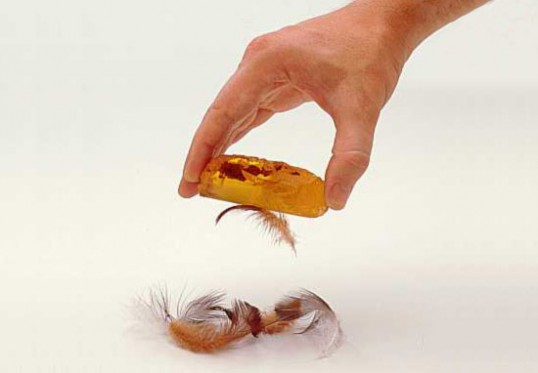
\includegraphics[width=0.7\linewidth]{Figuras/Ch01/ambar.JPG}}
}

\frame{
	\frametitle{Continuação das descobertas}
	\begin{block}{Willian Gilbert}
		\begin{itemize}
			\item Em 1600 o médico da rainha da Inglaterra denominou o evento de atração dos corpos de eletricidade.
			\item Publica “De Magnete”, onde explica que outros materiais, além do âmbar, adquiriam a propriedade de atrair outros corpos, e chamou a força observada de elétrica.
		\end{itemize}
	\end{block}

	\centerline{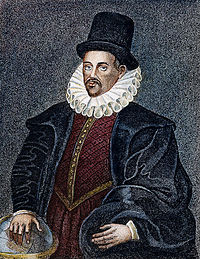
\includegraphics[width=0.25\linewidth]{Figuras/Ch01/gilbert.jpg}}
}

\frame{
	\frametitle{A eletricidade passa de um corpo para o outro?}
	\begin{block}{Otto Von Guericke}
		\begin{itemize}
			\item Em 1660, Otto Von Guericke, inventa a primeira máquina eletrostática, chamada de \textit{Elektrisiermaschine}. Era feita de uma esfera de enxofre atravessada por uma barra presa a uma manivela, que quando movimentada fazia a bola girar em alta velocidade. Otto protegeu a mão com uma luva que ao ser encostada na bola eletrizou-a instantaneamente. A bola começou a atrair outras bolas de enxofre suspensas por fios.
		\end{itemize}
	\end{block}

	\centerline{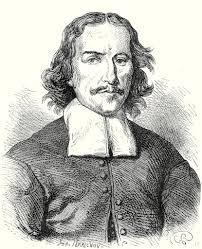
\includegraphics[width=0.25\linewidth]{Figuras/Ch01/otto.jpg}}
}

\frame{
	\frametitle{A eletricidade passa de um corpo para o outro?}
	\begin{block}{A máquina eletrostática de Otto}
		\begin{itemize}
			\item Otto conclui então que a eletricidade podia passar de um corpo para o outro.
			\item O que o levou a criar esse aparelho foram as pesquisas de Gilbert, sobre a eletrização por atrito.
		\end{itemize}
	\end{block}

	\centerline{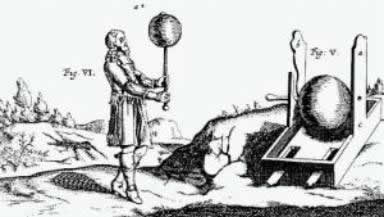
\includegraphics[width=0.65\linewidth]{Figuras/Ch01/otto2.jpg}}
}

\frame{
	\frametitle{Continuação da história}
	\begin{block}{Mais avanços...}
		\begin{itemize}
			\item 1675: Robert Boyle observa que as forças elétricas podem atuar através do vácuo.
			\item 1729: Stephen Gray fez a distinção entre materiais condutores e não condutores.
			\item 1730: Charles Francis Dufay descobriu que a eletricidade produzida por fricção podia ser de duas classes – positiva ou negativa.
		\end{itemize}
	\end{block}
}

\frame{
	\frametitle{A invenção dos pára-raios}
	\begin{block}{Charles Dufay}
		\begin{itemize}
			\item O químico francês Charles Dufay também contribuiu enormemente para o aprimoramento dos estudos da eletricidade, quando, em 1733, propôs a existência de dois tipos de eletricidade, a vítrea e a resinosa, que fomentaram a hipótese de existência de fluidos elétricos.
		\end{itemize}
	\end{block}

	\centerline{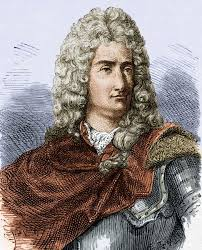
\includegraphics[width=0.3\linewidth]{Figuras/Ch01/dufay.jpg}}
}

\frame{
	\frametitle{A invenção dos pára-raios}
	\begin{block}{Benjamin Franklin}
		\begin{itemize}
			\item Essa teoria foi, mais tarde, por volta de 1750, continuada pelo conhecido físico e político Benjamin Franklin, que propôs uma teoria na qual tais fluidos seriam na verdade um único fluido. Baseado nessa teoria, pela primeira vez se conhecia os termos positivo e negativo na eletricidade.
		\end{itemize}
	\end{block}

	\centerline{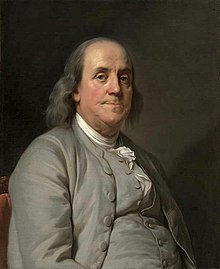
\includegraphics[width=0.3\linewidth]{Figuras/Ch01/benjamin.jpg}}
}

\frame{
	\frametitle{A invenção dos pára-raios}
	\begin{block}{A pipa de Franklin}
		\begin{itemize}
			\item Primeiro, Franklin demonstrou que o raio nada mais era do que uma faísca elétrica de uma nuvem positiva para a Terra negativa, ou vice-versa.
			\item Na linha da pipa, próximo a uma haste de metal, Franklin pendurou uma chave metálica. Quando a pipa estava próxima da base da nuvem, notou que pulavam faíscas da chave para a haste.
		\end{itemize}
	\end{block}

	\centerline{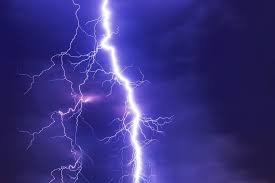
\includegraphics[width=0.5\linewidth]{Figuras/Ch01/raio.jpg}}
}

\frame{
	\frametitle{A invenção dos pára-raios}
	\begin{block}{A pipa de Franklin}
		\begin{itemize}
			\item Franklin pensou que se colocasse uma haste de metal bem alta, poderia descarregar a nuvem sem o raio. Daí o nome “para-raio”: ele inibiria o raio. Mas na verdade, o para-raio atrai o raio.
		\end{itemize}
	\end{block}

	\centerline{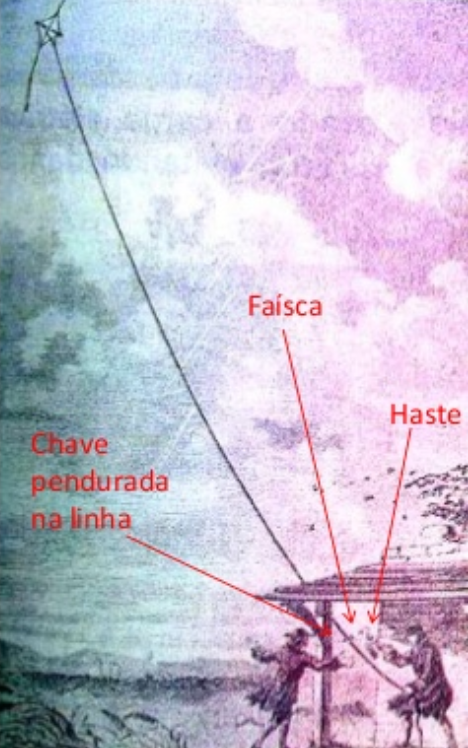
\includegraphics[width=0.27\linewidth]{Figuras/Ch01/pararaios.PNG}}
}

\frame{
	\frametitle{O surgimento da pilha}
	\begin{block}{Luigi Aloisio Galvani}
		\begin{itemize}
			\item Em 1780, Luigi Galvani, professor de Anatomia, descobre que as pernas de um sapo morto, que estava sobre uma placa metálica, sofriam uma contração quando tocadas com um bisturi.
			\item Durante um processo de dissecação, pendurou a perna de uma rã em um guincho de bronze preso a um poste de ferro. Durante uma tempestade, observou que a faísca elétrica a fazia saltar.
		\end{itemize}
	\end{block}

	\centerline{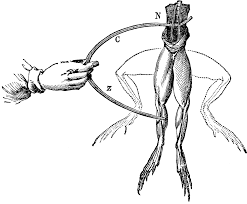
\includegraphics[width=0.35\linewidth]{Figuras/Ch01/ra.png}}
}

\frame{
	\frametitle{O surgimento da pilha}
	\begin{block}{Alessandro Volta}
		\begin{itemize}
			\item O seu trabalho foi compartilhado e a sua ideia desdobrada, sendo imprescindível na criação de Alessandro Volta, a Pilha Voltaica (1800).
			\item O italiano Alessandro Volta, descobre que ocorre uma reação química quando dois metais diferentes entram em contato com uma solução ácida. Devido a esta reação surge uma corrente elétrica.
		\end{itemize}
	\end{block}

	\centerline{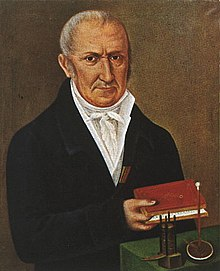
\includegraphics[width=0.27\linewidth]{Figuras/Ch01/volta.jpeg}}
}

\frame{
	\frametitle{O surgimento da pilha}
	\begin{block}{A pilha de Volta}
		\begin{itemize}
			\item Volta construiu a primeira pilha utilizando discos de cobre e zinco, separados por um material que continha uma solução ácida.
		\end{itemize}
	\end{block}

	\centerline{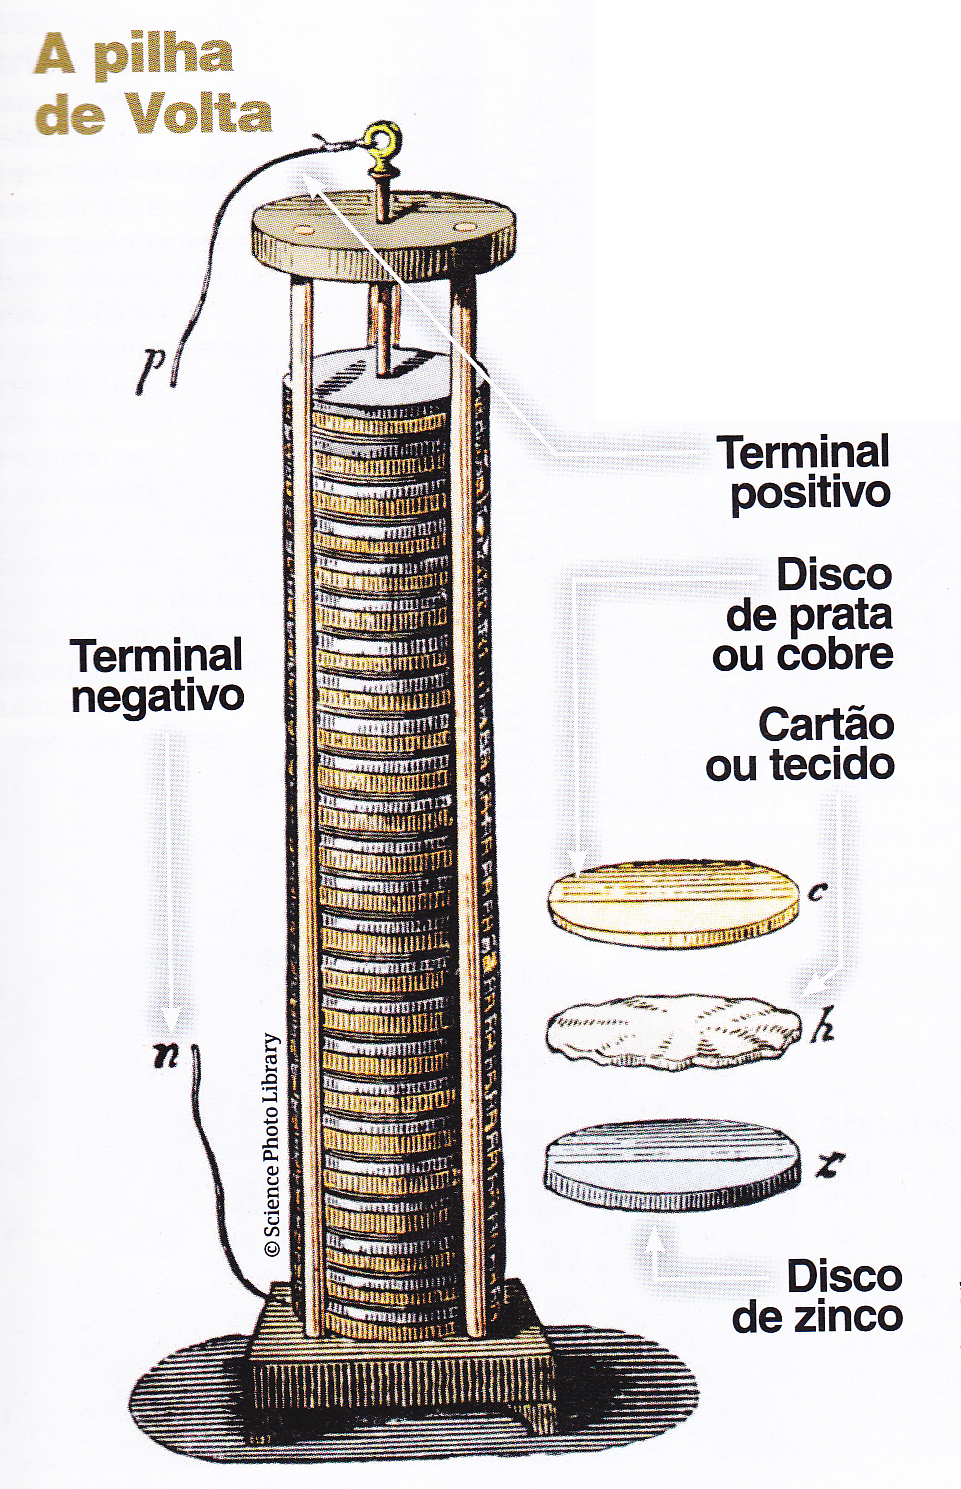
\includegraphics[width=0.32\linewidth]{Figuras/Ch01/pilha.png}}
}

\frame{
	\frametitle{Eletromagnetismo}
	\begin{block}{Hans Christian Oersted}
		\begin{itemize}
			\item Em 1820, na Dinamarca, Hans Christian Oersted descobre que uma corrente elétrica fluindo num condutor é capaz de alterar a agulha de uma bússola. Esta observação fica conhecida como o Experimento de Oersted.
			\item Com isso, percebe-se que há uma ligação entre magnetismo e eletricidade.
		\end{itemize}
	\end{block}

	\medskip
	
	\centerline{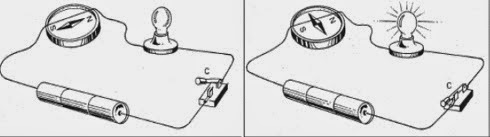
\includegraphics[width=0.9\linewidth]{Figuras/Ch01/oersted.jpg}}
}

\frame{
	\frametitle{Eletromagnetismo}
	\begin{block}{Solenoide}
		\begin{itemize}
			\item Em 1820, na França, André Maria Ampere demonstrou que condutores percorridos por correntes elétricas desenvolvem forças de atração ou de repulsão. Ele inventou o solenoide.
			\item Em 1827, Ampere elaborou a fórmula matemática do eletromagnetismo, a conhecida ``Lei de Ampere''.
		\end{itemize}
	\end{block}

	\centerline{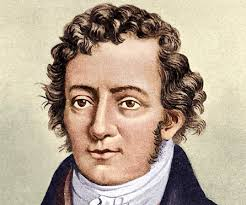
\includegraphics[width=0.4\linewidth]{Figuras/Ch01/ampere.jpg}}
}

\frame{
	\frametitle{Eletromagnetismo}
	\begin{block}{Michael Faraday}
		\begin{itemize}
			\item Em 1831, Michael Faraday descobre que a variação na intensidade da corrente elétrica que percorre um circuito fechado induz uma corrente em uma bobina próxima. Uma corrente induzida também é observada ao se introduzir um ímã nessa bobina. Essa indução magnética teve uma imediata aplicação na geração de correntes elétricas.
		\end{itemize}
	\end{block}

	\centerline{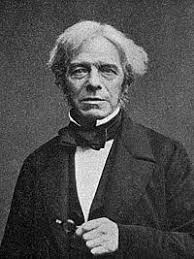
\includegraphics[width=0.25\linewidth]{Figuras/Ch01/faraday.jpg}}
}

\frame{
	\frametitle{Eletromagnetismo}
	\begin{block}{Lei de Faraday}
		\begin{itemize}
			\item Uma bobina próxima a um ímã que gira é um exemplo de um gerador de corrente elétrica alternada.
		\end{itemize}
	\end{block}

	\vspace{0.2cm}

	\centerline{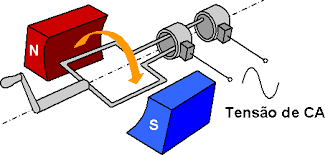
\includegraphics[width=0.8\linewidth]{Figuras/Ch01/geracaoca.png}}
}

\frame{
	\frametitle{Telégrafo e máquinas elétricas}
	\begin{block}{Telégrafo eletromagnético}
		\begin{itemize}
			\item No ano de 1833, na Alemanha, Wilhelm Weber e Karl Gauss desenvolveram um telégrafo eletromagnético que posteriormente foi aperfeiçoado por Werner Von Siemens e Samuel Morse.
			\item No mesmo ano em Inglaterra Michael Faraday estabeleceu as leis da eletrólise, da capacidade elétrica e inventou o motor elétrico, o dínamo e o transformador.
		\end{itemize}
	\end{block}
}

\frame{
	\frametitle{Iluminação}
	\begin{block}{Thomas Edison}
		\begin{itemize}
			\item Em 1830, nos Estados Unidos, Joseph Henry descobriu a “indução eletromagnética” e a conversão do magnetismo em eletricidade.
			\item E em 1880, nos Estados Unidos, Thomas Edison desenvolveu a lâmpada elétrica incandescente.
		\end{itemize}
	\end{block}

	\centerline{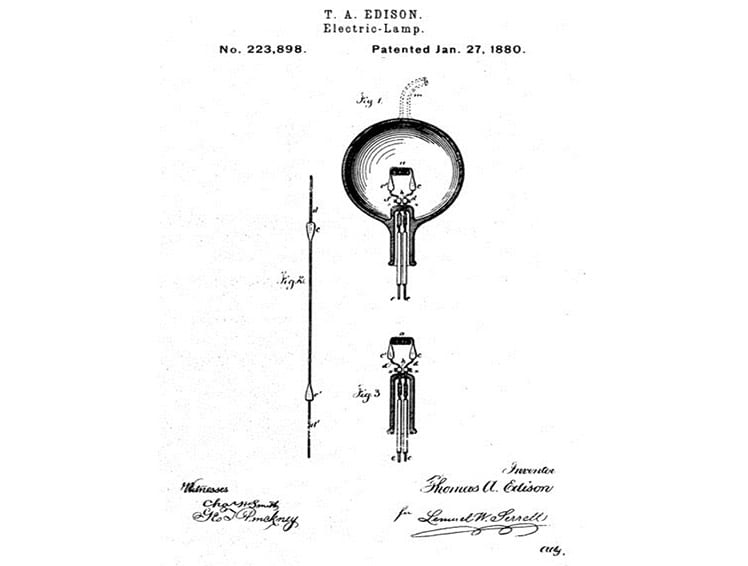
\includegraphics[width=0.5\linewidth]{Figuras/Ch01/lampada.jpg}}
}

\frame{
	\frametitle{Geração de energia elétrica}
	\begin{block}{Leis de Maxwell}
		\begin{itemize}
			\item Em 1864, na Inglaterra, James Maxwell desenvolveu as equações fundamentais do eletromagnetismo: as Leis de Maxwell.
			\item A Publicação do tratado sobre eletricidade e magnetismo, de James Clerk Maxwell, em 1873, representa um enorme avanço no estudo do eletromagnetismo. A luz passa a ser estendida como onda eletromagnética,
			\item Em 1882, Thomas Edison, projetou e construiu as primeiras máquinas geradoras, uma em Londres e duas nos Estados Unidos. Ambas eram de pequeno porte e forneciam eletricidade em corrente contínua.
		\end{itemize}
	\end{block}
}

\frame{
	\frametitle{Corrente alternada}
	\begin{block}{George Westhinghouse}
		\begin{itemize}
			\item Em 1886, nos Estados Unidos, George Westhinghouse inaugurou o primeiro sistema de energia elétrica na Califórnia utilizando um transformador eficiente desenvolvido por William Stanley.
			\item No ano de 1887, já havia algumas máquinas na Califórnia que alimentavam cerca de \num{135000} lâmpadas. A transmissão era feita em 1000 volts.
		\end{itemize}
	\end{block}

	\centerline{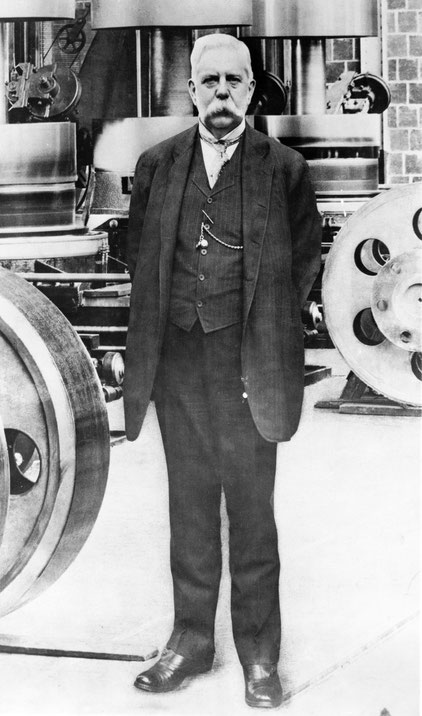
\includegraphics[width=0.2\linewidth]{Figuras/Ch01/george.jpg}}
}

\frame{
	\frametitle{Corrente alternada}
	\begin{block}{Nikola Tesla}
		\begin{itemize}
			\item Em 1890, na Sérvia, Nikola Tesla criou o sistema de geração de energia elétrica trifásico, que passou a ser utilizado em 1896.
		\end{itemize}
	\end{block}

	\centerline{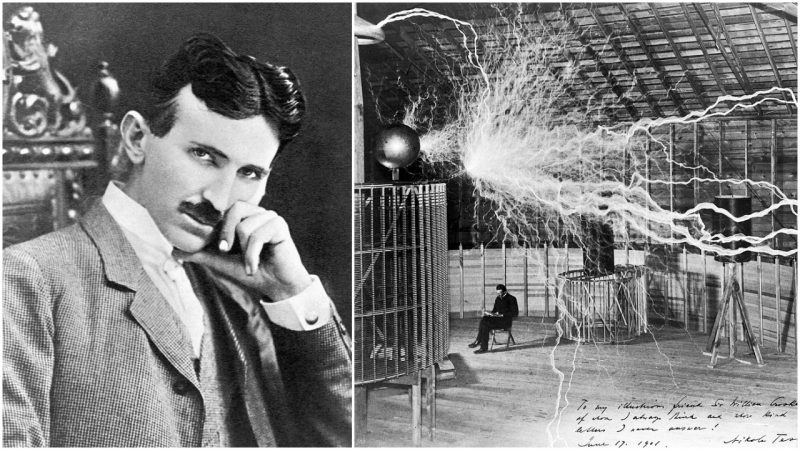
\includegraphics[width=0.7\linewidth]{Figuras/Ch01/tesla.jpg}}
}

\frame{
	\frametitle{A guerra das correntes}
	\begin{block}{Nikola Tesla vs. Thomas Edison}
		\begin{itemize}
			\item A guerra das correntes foi uma disputa entre Nikola Tesla e Thomas Edison que ocorreu nas duas últimas décadas do século XIX. Os dois tornaram-se adversários devido à campanha publicitária de Edison pela utilização da corrente contínua para distribuição de eletricidade, em contraposição à corrente alternada, defendida por Westinghouse e Nikola Tesla.
		\end{itemize}
	\end{block}

	\centerline{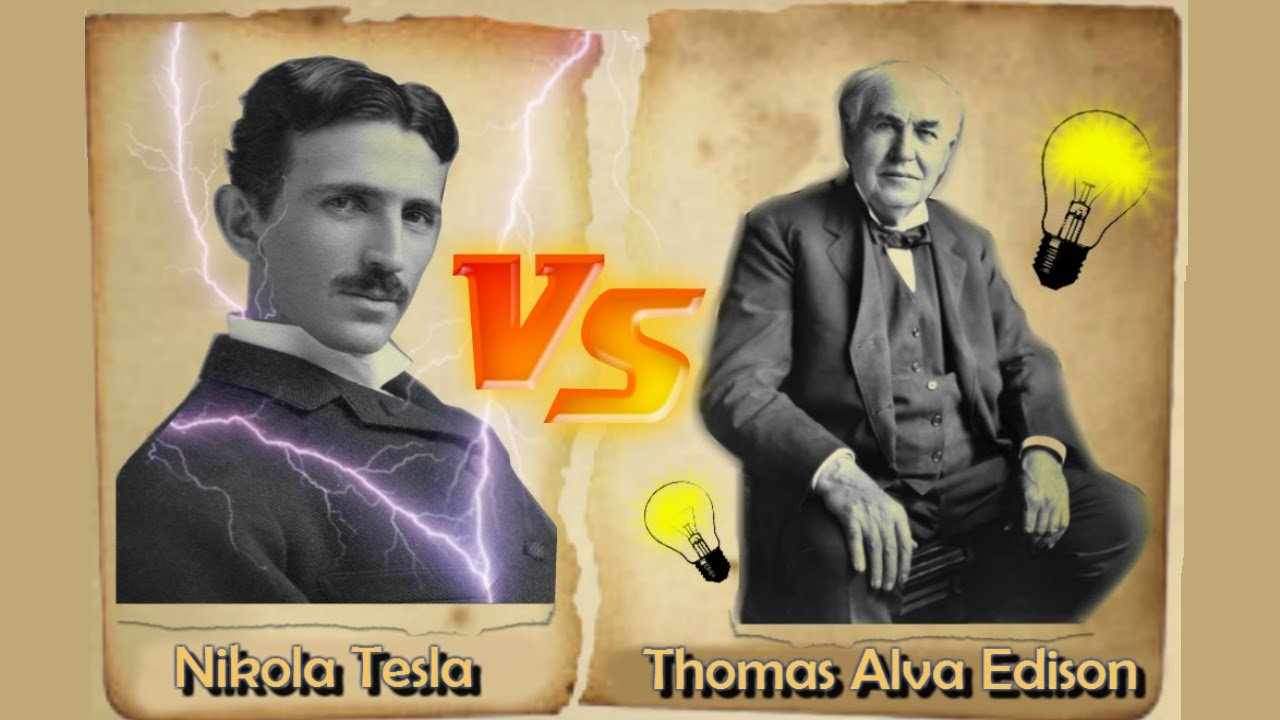
\includegraphics[width=0.6\linewidth]{Figuras/Ch01/guerra.jpg}}
}

\frame{
	\frametitle{A guerra das correntes}
	\begin{block}{Os motivos}
		\begin{itemize}
			\item Havia diversas explicações para essa rivalidade: Edison era um experimentador voraz, mas não era matemático. A corrente alternada não pode ser devidamente entendida ou aproveitada sem um conhecimento substancial de matemática e física, o que Tesla possuía.
			\item Tesla havia trabalhado para Edison, mas foi subestimado (por exemplo, quando soube das ideias de Tesla da transmissão de energia por corrente alternada, Edison recusou-as: ``As ideias (de Tesla) são magníficas, mas não são nada práticas''.
			\item Maus sentimentos foram exacerbados quando Tesla foi enganado por Edison, que prometeu-lhe uma recompensa por seu trabalho.
			\item Edison, mais tarde, teria se arrependido, por não ter ouvido Tesla e utilizado corrente alternada.
		\end{itemize}
	\end{block}
}

\frame{
	\frametitle{A eletricidade}
	\begin{block}{Definição}
		\begin{itemize}
			\item A eletricidade é a área da Física responsável pelo estudo de fenômenos associados a cargas elétricas.
		\end{itemize}
	\end{block}

	\centerline{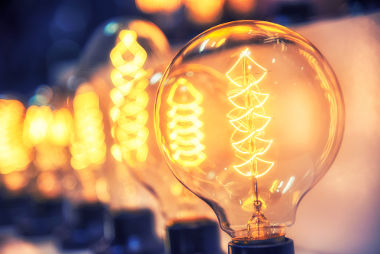
\includegraphics[width=0.6\linewidth]{Figuras/Ch01/eletricidade.jpg}}
}

\frame{
	\frametitle{A eletricidade}
	\begin{block}{Divisão}
		\begin{itemize}
			\item \textbf{Eletrostática}: refere-se ao comportamento das cargas elétricas em repouso e seu estudo engloba os processos de eletrização, campo elétrico, força eletrostática e potencial elétrico.
			      \vspace{0.5cm}
			\item \textbf{Eletrodinâmica}: é a parte da eletricidade responsável pelo estudo das cargas elétricas em movimento. O foco dessa área é a corrente elétrica e os componentes de circuitos elétricos, como capacitores e resistores.
			      \vspace{0.5cm}
			\item \textbf{Eletromagnetismo}: estuda a relação entre os fenômenos elétricos e magnéticos, tais como campo magnético produzido por cargas elétricas em movimento e campo elétrico produzido pela variação de fluxo magnético.
		\end{itemize}
	\end{block}
}

\section*{Exercícios}

\frame{
	\frametitle{Exercícios}
	\begin{block}{}
		01. A respeito do desenvolvimento dos estudos relacionados com o magnetismo, marque V para as afirmações verdadeiras e F para as falsas.

		\vspace{0.5cm}

		(  ) Os primeiros estudos realizados na área do magnetismo foram feitos por Aristóteles no século VI a.C. O filósofo analisou a atração entre pedras de um minério denominado de magnetita.

		\vspace{0.5cm}

		(  ) A utilização da bússola provavelmente foi a primeira aplicação prática do magnetismo.

		\vspace{0.5cm}

		(  ) A relação entre magnetismo e eletricidade só foi aceita no século XX com os estudos de Michael Faraday.

		\vspace{0.5cm}

		(  ) O experimento de Oersted, realizado no século XIX, abriu caminho para os estudos relacionados ao eletromagnetismo.
	\end{block}
}

\section*{Referências}

\frame{
	\frametitle{Referências e Exercícios Complementares}
	\begin{itemize}
		\item Física, Ciência e Tecnologia – Vol 3. PENTEADO, Paulo César M; TORRES, Carlos Magno A. Ed. Moderna (2006)
	\end{itemize}
	%\centering{\alert{Página 36 - \textbf{1.6.1 até 1.6.5, 1.6.17 até 1.6.19}}} \\
	%https://www.youtube.com/watch?v=IUgS7Uw-qBI
	\centering{\alert{Lista de exercícios 01}}
}
